
In this chapter, we present the state-of-the-art of this thesis. We discuss previous efforts in three research areas: (1) Compiler auto-tuning in iterative compilation, (2) code generator testing, and (3) container-based testing.

We first present a brief introduction to the iterative compilation research filed and we identify severals problems that have been investigated in this field. We discuss as well, the different techniques that have been applied to automate the process of auto-tuning compilers. To sum up, we provide a summary table showing the most important research in iterative compilation.

Afterwards, we move to discuss existing techniques related to code generator testing. We start by studying the state-of-the-art approaches related to the functional testing of code generators. In a second stage, since there are few research efforts that investigate the automatic non-functional testing of code generators, we rather focus on studying the oracle problem and the different methods applied to the oracle definition. This will be useful later, to understand our contribution about the non-functional testing of code generators. We end this section by providing a summary table of these approaches.

Finally, we discuss in the last section the container technology as means of automatic software deployment, monitoring, and testing. We compare then, the container's virtualization solution to the classical approaches based on virtual machines. We provide as well, examples of existing solutions in research and industry that opted for this technology to automate software testing and monitoring.

This chapter is structured as follows: Section 3.1 provides a survey of the most used compiler auto-tuning techniques to construct the best set of optimization options. In Section 3.2, we review existing techniques for code generators testing and the principal categories of oracles. Then, in Section 3.3, we discuss the use of virtualization technology for deployment and testing. In particular, we presents some of the approaches that used a container-based solution for automatic testing and monitoring. Finally, Section 3.3 discusses the limitations of the state of the art.
\section{Compilers auto-tuning techniques}

\subsection{Iterative compilation}
Iterative compilation, \textit{also known by optimization phase selection, adaptive compilation, or feedback directed optimization}, consists in applying software engineering techniques to produce better and more optimized programs by compiling multiple versions of each of them using different optimizations settings. After running these versions on specific hardware machines, the key objective of iterative compilation is to find the best optimizing sequence that leads to the fastest and better code machine code. 
Our work is related to iterative compilation research field.
The basic idea of iterative compilation is to explore the compiler optimization space by measuring the impact of optimizations on software performance.
Several research efforts have investigated this optimization problem using Search-Based Software Engineering (SBSE) techniques to guide the search towards relevant optimizations regrading performance, energy consumption, code size, compilation time, etc. Experimental results have been usually compared to standard compiler optimization levels.  

It has been proven that optimizations are highly dependent on the target platform and on the input program. 
Compared to our proposal, none of the previous work has studied the impact of compiler optimizations on resource usage. In this work, we rather focus on compiler optimizations related to resource consumption, while bearing in mind the performance improvement.

\subsection{Implementation of iterative compilation system}
\begin{figure}[h]
	\center
	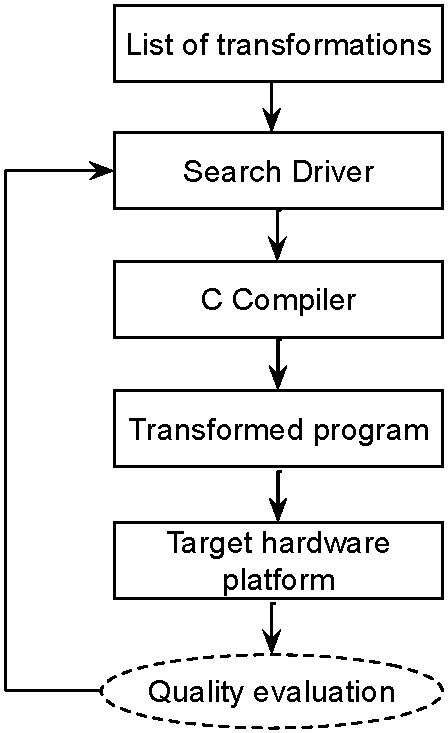
\includegraphics[scale=0.65]{SOTA/fig/iterative_compilation}
	\caption{Overview of the iterative compilation process}
	\label{fig:iterative_compilation}
\end{figure}
The implementation of an iterative compilation system consists mainly on applying a sequence of steps to enhance the quality of the generated code. Figure~\ref{fig:iterative_compilation} shows a general overview of the main steps needed to ensure the implementation of the iterative compilation process.
\begin{itemize}
	\item[--] \textbf{List of transformations:}
	
	The iterative process starts by defining the optimization space. It represents the list of optimizations that the compiler have to evolve during the search to enhance the software quality.
	
	\item[--] \textbf{Search driver:}
	
	It applies a search algorithm or method to efficiently explore the large optimization search space. In fact, it reads the previously defined list of transformations that it needs to examine and decides which transformations have to be applied next using a search algorithm
	to steer through the optimization space.
	
	\item[--] \textbf{C Compiler:}
	
	Once the optimization sequence is defined, the target C compiler is called to compile the input program and also perform initial machine independent optimizations. 
	
	\item[--] \textbf{Transformed program:}
	
	This results in an initial machine independent optimized program. These optimizations are performed during code generation and impact all target systems. It includes optimizations that are applied during the parse tree mapping to the intermediate code and the optimization applied to the intermediate code itself.
	
	\item[--] \textbf{Target hardware platform:}
	
	For further optimization, the compiler applies from the provided optimization sequence the machine dependent optimizations. They are specific to the object code being generated. This includes optimizations applied during the mapping of intermediate code to assembler and optimizations applied directly on the generated object code.
	
	\item[--] \textbf{Quality evaluation:}
	
	It consists on evaluating the quality of the optimized code. Many non-functional properties can be evaluated like code size, execution time, resource usage, power consumption, etc.
	
\end{itemize}

This model represents the classical and typical iterative compilation process. Of course, there exist many ways and adaptations to implement this process. The implementation of the iterative process depends on the algorithm used, the problem addressed, the technologies used, etc. The goal of the next sub-sections is to present the different state-of-the-art approaches related to iterative compilation.

\subsection{Iterative compilation search techniques}
In Section 2.5.2 of Chapter 2, we presented several issues with optimizing compilers that make the activity of compiler tuning very complex such as the huge number of optimizations, conflicting objectives, optimization overhead, etc.
In this section, we discuss the available tools and approaches dedicated to the automatic search for optimal compiler settings, and give an overview of known approaches that addressed the several compiler optimization challenges. In each subsection, we identify and discuss a particular problem and we present the best known approaches proposed to solve it.

\subsubsection{Auto-tuning: a mono objective optimization}
Auto-tuning is an area that study of automatic code generation and optimization for different computer architectures.
This technique has been used in many optimization scenarios.
What all of this prior work on iterative compilation has in common is that it focuses on a single objective function to be optimized. For example, researchers typically focus on speeding up the performance of compiled code which constitutes the major optimization objective for most iterative compilation approaches\cite{pan2006fast,haneda2005automatic}. 

So, the problem has been often adapted as a mono-objective search problem where the speedup is the main concern for most of the previous works. 
Genetic algorithms (GA)\cite{stephenson2003genetic,bashkansky2007black} present an attractive solution to this problem of selecting an optimal set of options. 
GA-based approaches compute an initial population using a set of optimizations, generally defined under the standard compiler levels Ox. Then, at each iteration, the individuals (i.e., option sets) that comprise the generation are evaluated by measuring the execution time resulted by a specific set of options. The results are sorted and pass through a breeding and mutation stage to form the next generation. This
process continues until a termination condition is reached. The algorithm returns the best optimization set that led to the highest performance.

For example, ACOVEA \footnote{https://github.com/Acovea/libacovea} as Analysis of Compiler Options via Evolutionary Algorithm, is an open source tool that utilize genetic algorithms to find the best options for compiling programs with the GNU Compiler Collection (GCC) C and C++ compilers. In this context, best solutions define those options that produce the fastest executable program from a given source code. This tool was even included in Gentoo Linux
repository to help users to find their best set of optimizations.

As an example, the ESTO framework described in \cite{bashkansky2007black} studies the application of GA for the problem of selecting an optimal option set for a specific application and workload. It searches the option set space using various types of genetic algorithms, ultimately determining the option set that maximizes the performance of the given application and workload. ESTO regards the compiler as a black box, specified by its external-visible optimization options. ESTO supports also a GA variant named budget-limited genetic algorithm which reduces the population size exponentially and then reduce the time needed to evaluate the different evaluations. They ran experiments on the SPEC2000 benchmark suite and tested 60 optimization options within three compilers: GCC, XLC and FDPR-Pro. Results of ESTO are compared to GCC -O1 and -O3, to XLC -O3 and to FDPR-Pro -O3. The results show that ESTO is capable to construct optimization levels that yield to better performance than standard options.

Most the approaches described above focus on auto-tuning compilers without putting too much emphases on the tuning time. The process of auto-tuning may be too long and can last more than one month\cite{hoste2008cole}.

As a consequence, Pan et al.\cite{pan2006fast} introduce a new algorithm called combined elimination (CE) that was shown to outperform all previous search-based techniques in finding good optimization settings with considerably fewer evaluations. The proposed solution, PEAK, achieves fast tuning speed by measuring a small number of invocations of each code section, instead of the whole-program execution time, as in common solutions. Compared to these solutions PEAK reduces tuning time from 2.19 hours to 5.85 minutes on average, while achieving similar program performance.
PEAK improves the performance of SPEC CPU2000 FP benchmarks by 12\% on average over GCC O3, the highest optimization level, on a Pentium IV machine.


%\subsubsection{JIT compiler optimization}

%\subsubsection{Dealing with numerical parameter values}
%The phase ordering problem is a common problem in iterative compilation. It is related to numerical parameters optimization where the parameter optimization value should be determined automatically.

\subsubsection{Escaping local optimum}


A common problem in iterative compilation is the local optimum. In fact, the search space of optimizations for a specific program could be very huge and it generally contains many local minima in where the search algorithm could be trapped\cite{bodin1998iterative}. Therefore, researchers in this filed try to build robust techniques and algorithms to avoid such problem.
In \cite{bodin1998iterative}, Bodin et al. tried to analyze this search space and they found that the optimization space is highly non-linear containing many local minima and some discontinuities. Therefore, techniques based on gradient approaches such as GAs are not applicable.
This paper has focused on parameterized transformations. The small area of the transformation space considered in this paper is composed by three parameterized optimizations: loop unrolling (with unroll factors from 1 to 20), loop tiling (with tile sizes from 1 to 100) and padding (from 1 to 100). They focused on compilation time and execution time of the optimized program and used a simulator to target embedded processors. The compiler used is a compiler framework developed to optimise multimedia codes for embedded systems.
They analyzed these optimizations on four CPU architectures (UltraSparc, R10000, Pentium Pro, and TriMedia-1000) and the matrix multiplication is selected as the program to optimize.
The proposed search algorithm visits a number of points at spaced intervals, applying the appropriate transformation, executing
the transformed program and evaluating its worth by measuring the execution time. Those points lying between
the current global minimum and the average are added to an ordered queue. Iteratively, such points are removed from the queue and points within the neighboring region are investigated, again at spaced intervals. This process is continued until a specific number of points have been evaluated and the fastest transformed program is reported.
They showed that in the case of large transformation spaces, they can achieve within 0.3\% of the best possible time by visiting less then 0.25\% of the space using a simple algorithm and find the minimum after visiting up to less than 1\% of the space.

Cooper et al.\cite{cooper2006exploring} describe their experience exploring the search space of compilation sequences. They give results for exhaustively enumerating several search spaces of sequences of length 10 chosen from 5 transformations. They show that the search spaces have many local minimum, and that random-restart hill climbing is an effective strategy to overcome shallow local minima.

%paper: Exhaustive Optimization Phase Order Space Exploration
%Earlier work in iterative compilation concentrated on finding good parameter settings for a few optimizations, such as loop unrolling and loop tiling\cite{bodin1998iterative}. In cases where exhaustive exploration was expensive, researchers
%used heuristic algorithms, such as grid-based searches, hill climbers, and genetic algorithms, to scan only a portion of the search space. A common deduction is that typical program search spaces, on a variety of different architectures, generally contain enough local minima that biased sampling techniques should find good solutions.

\subsubsection{Phase ordering problem}
Phase ordering is also an important problem in iterative compilation which explores the effect of different orderings of optimization phases on program performance. In fact, when using some compilers such as LLVM, it is important to define the right order of applying optimizations. Thus, researchers in this field try to apply search techniques in order to find the right optimization sequence. However, reordering optimization phases is extremely hard to support in most production systems, including GCC due to their use of multiple intermediate formats and complex inherent dependencies between optimizations. So generally, compilers manage internally the order of applying optimizations and do not give the hand to the user to choose this order to avoid conflicts and compilation issues.

When the order is managed by the users, exhaustively evaluating  all orderings of optimization phases is infeasible in the face of a huge number optimization phases. This problem becomes more complex by the fact that these phases interact with other optimizations in a complex way.
For example, even if we keep the same set of optimizations for an input program, varying the order of applying these optimization phases can produce different code, with potentially significant performance variation amongst them. 

In this trend, Whitfield developed a framework based on axiomatic specifications of optimizations and includes both pre and post conditions that must exist before and after applying optimizations\cite{whitfield1990approach}. For a selected set of optimizations, the framework is used to determine those interactions among the optimizations that can create conditions and those that can destroy conditions for applying other optimizations. Then, from these interactions, an application order is derived to obtain the potential benefits of the optimizations that can be applied to a program. 
This framework was employed to list the potential enabling and disabling interactions between optimizations, which were then used to derive an application
order for the optimizations

Kulkarni et al.\cite{kulkarni2009practical,kulkarni2006exhaustive} proposed an exhaustive search strategy to find optimal compilation sequences for each function of a program. They exhaustively enumerated all distinct function instances for a set of programs that would be produced from different phase-orderings of 15 optimizations. This exhaustive enumeration was made possible by detecting which phases were active and whether or not the generated code was unique, making the actual optimization phase order space much smaller than the attempted space. This exhaustive enumeration allowed them to construct probabilities of enabling/disabling interactions between different optimization passes in general and not specific to any program. They use this idea to prevent the combinatorial explosion of the total number of sequences to be tested. 
This exhaustive enumeration allowed them to construct probabilities of enabling/disabling interactions between different optimization passes in general and not specific to any program. 
They were able to find all possible function instances that can be produced by different phase orderings for 109 out of the 111 total functions they evaluated.


Several researchers looked at searching for the best sequence of optimizations for a particular program. For example, the work of Cooper et al.\cite{cooper1999optimizing} adapts the genetic algorithm to solve the optimization phase ordering problem. The focus of this paper is about optimizing for embedded systems and then reducing the code size. They choose 10 program transformations to evolve in Fortran compiler. The solutions generated by this algorithm are compared to solutions found using a fixed optimization sequence and solutions found by testing random optimization sequences. Their technique was successful for reducing the code size by 40\% compared to the standard sequence.

In another work\cite{cooper2006exploring} the same authors explored phase orders at program-level with randomized search algorithms based on genetic algorithms, hill climbers and randomized sampling. They target a simulated abstract RISC-based processor with a research compiler, and report properties of several of the generated sub-spaces of phase ordering and the consequences of those properties for the search algorithms.

\subsubsection{Evaluating iterative optimization across multiple data sets}
Most iterative optimization studies find the best compiler optimizations through repeated runs on input program and the same data set. The problem is that if we select the best optimization sequence for an input data set through the iterative process, we do not know if it will still be the best for the same program but with other data sets. Thereby, researchers in this field try to investigate this problem by evaluating the effectiveness of iterative optimization across a large number of data sets. In particular, since there is no existing benchmark suite with a large number of data sets  Chen et al.\cite{chen2010evaluating} attempt to collect 1000 data sets called KDataSets for 32 programs, mostly derived from the MiBench benchmark. Then, they exercise iterative optimization on these collected data sets in order to fin the best optimization combination across all data sets. 
They use random search to generate random optimization sequences for the ICC compiler (53 flags) and the GCC compiler (132 optimizations).
They demonstrate that for all 32 programs (from MiBench), they were able to find at least one combination of compiler optimizations that achieves 86\% or more of the best possible speedup across all data sets using Intel’s ICC (83\% for GNU’s GCC). This optimal combination is program-specific and yields speedups up to 1.71 on ICC and 2.23 on GCC over the highest optimization level (-fast and -O3, respectively). This means that a program can be optimized on a collection of data sets and it can retain near optimal performance for most other data sets. So the problem of finding the best optimization for a particular program may be significantly less complex. However, they tested their approach on only one single benchmark and one target architecture.




\subsubsection{Conflicting objectives: a multi-objective optimization}
The vast majority of the work on iterative compilation focuses on increasing the speedup of new optimized code compared to standard compiler optimization levels. However, they do not put too much emphasis on finding trade-offs between two (or more) non-functional properties ~\cite{almagor2004finding,hoste2008cole,pan2006fast,pallister2015identifying,chen2012deconstructing,martins2014exploration,lin2008automatic,martinez2014multi}.

In COLE\cite{hoste2008cole}, the authors considered that the problem of compiler optimizations can be seen as a multi-objective problem where two non-functional properties can be enhanced simultaneously. Thus, they investigated the standard levels of compiler optimization by searching for Pareto optimal levels that maximize both performance and compile time. 
They show that by using the multi-objective genetic algorithm (in their experiment they used SPEA2), it is possible to find a set of compiler optimization sequences that are more Pareto-effective in terms of performance and compile time than the standard optimization levels (-O1, -O2, -O3, and -Os). The motivation behind this approach is that these standard levels were set up manually by compiler creators based on fixed benchmarks and data sets. For the authors, these universal levels may not be always effective on unseen programs and there exist higher levels that provide better trade offs in terms of code quality.
The authors used the SPEC2000 CPU benchmark, which is a popular benchmark suite for evaluating the compiler performance. They evolved 60 optimization flags that are defined in the standard levels O1, O2, O3, O1 and OS. They run iterative compilation on one single machine shipped with Intel CPU Pentium 4 and they compared the proposed algorithm (SPEA2) to random search as well as to standard optimization levels.

The experimental results using GCC (v4.1.2) show that the automatic construction of optimization levels is feasible in practice, and in addition, yields better optimization levels than GCC’s manually derived (-Os, -O1, -O2 and -O3) optimization levels, as well as the optimization levels obtained through random sampling.
However, They do not provide a guarantee that the new explored optimization levels selected for SPEC still will be optimal for other applications.


Martinez et al.\cite{martinez2014multi} propose an adaptive worst-case execution time WCET-aware compiler framework for automatic search of compiler optimization sequences which yield highly optimized code. 
Compared to the previously described approaches, authors in this paper focus on generating efficient code for embedded systems. Embedded systems are characterized by both efficiency requirements and critical timing constraints. Properties as average-case performance, power consumption and resource utilization are the main concerns describing the efficiency of a system. 
Thus, they explore the performance of compiler optimizations with conflicting goals. 
Besides the objective functions average-case execution time and code size, they consider the WCET, which is a crucial parameter for real-time systems, especially for
safety-critical application domains such as automotive and
avionics to avoid system failure. 
Then, they try to find suitable trade-offs between these objectives in order to identify Pareto optimal solutions using stochastic evolutionary multi-objective algorithms. The objective functions try to minimize the WCET-ACET and WCET-Code size properties. They apply three evolutionary multi-objective algorithms (EMO) namely IBEA, NSGA-II and SPEA2 and compare their results to standard levels (O1, O2 and O3). 
They evolve 30 optimizations within the WCC compiler and performed experiments on top of one single machine shipped with Intel Quad-Core CPU processor. They pick up as well 35  programs from various benchmarks such as DSPstone, MediaBench, MiBench, etc.
They find that NSGA-II is the most promising EMO for the given problem. In fact, the discovered optimization sequences significantly outperform standard optimization levels:
the highest standard optimization level O3 can be outperformed for the WCET and ACET on average by up to 31.33\% and 27.43\%, respectively. The same approach performs as well for the WCET-Code size optimization with a 30.6\% WCET reduction over O3. However, the code size increases by 133.4\%. This is because the WCET and the code size are typical conflicting goals. If a high improvement of one objective function is desired, a significant degradation of the other objective must be accepted.

In \cite{plotnikov2013automatic}, the TACT framework is presented. 
Compared to previous approaches, TACT is designed primarily for automatic tuning on embedded systems running Linux. Thus, the target CPU architecture for this tool is the ARM architecture (ARM Cortex-A9) and 200 options are used in the GCC compiler for ARM. 

TACT supports multiple optimization objectives, so it can tune either for a single optimization parameter, or for two objective functions simultaneously, for example, for performance and code size (or compile time). So, it applies the SPEA2 algorithm and GA for mono-objective optimizations.

The results show how the SPEA2 outperforms the standard GCC levels (O2, O3 and Os) across several open-source popular applications such as  C-Ray, Crafty Chess, SciMark, x264 and zlib.


 

\subsubsection{Predicting optimizations: a machine learning optimization}
Machine learning has been also proposed by several research efforts to tune optimizations across programs. Compared to evolutionary algorithms, using machine learning in compiler optimization has the potential of reusing knowledge across the different iterative compilation runs, gaining the benefits of iterative compilation to learn the best optimizations across multiple programs and architectures.

Generally, machine learning techniques create mainly in an off line phase a prediction model, which will be used to determine the compiler optimization set that should be used on a test (unseen) program by the online phase. The main advantage of this technique is that it reduces the number of required program evaluations.

In the Milepost project\cite{fursin2011milepost} for example, authors start from the observation that similar programs may exhibit similar behavior and require similar optimizations, so it is possible to correlate program features and optimizations together to predict good transformations for unseen programs, based on previous optimization experience. Thereby, they provide a modular, extensible, self-tuning optimization infrastructure that can automatically learn how to best optimize programs for configurable heterogeneous processors based on the correlation between program features, run-time behavior and optimizations. 

The proposed infrastructure is based on a machine learning compiler that presents an Interactive Compilation Interface (ICI) and plugins to extract program features (such as the number of instructions in a method, number of branches, etc) and select optimization passes. 

The Milepost framework proceeds in two distinct phases: training and deployment. During the training phase, information about the structure of programs (input training programs) is gathered, showing how they behave under different optimization settings. Such information allows machine learning tools to correlate aspects of program structure, or features, with optimizations, building a strategy that predicts good combinations of optimizations. 
After running an iterative process that evaluates different combinations of optimizations on top of the training programs/features, pedictive models are created to correlate a given set of program features with profitable program transformations. 
Then, in the deployment phase, the framework analyzes new unseen programs by determining the program features and passes them to the new created models to predict the most profitable optimizations to improve execution time or other metrics depending on the user’s optimization requirements.

GCC was selected as the compiler infrastructure for Milepost as it is currently the most stable and robust open-source compiler. They evolved 100 optimization flags under O1, O2 and O3 levels and compared their results to the O3 level and to the random search.

The experimental results show that it is possible to improve the performance of the MiBench benchmark suite automatically using iterative compilation and machine learning on several platforms, including x86: Intel and AMD, and the ARC configurable core family. Using the machine learning-based framework, they were also able to learn a model that automatically improves the execution time of some individual MiBench programs by a factor of more than 2 while improving the overall MiBench suite by 11\% on reconfigurable ARC architecture, without sacrificing code size or compilation time. Furthermore, their approach supports general multi-objective optimization where a user can choose to minimize not only execution time but also code size and compilation time.



\subsubsection{Summary: auto-tuning compiler techniques}
 


\section{Testing code generators}
\subsection{Testing functional properties}


Most of the previous work on code generators testing focuses on checking the correct functional behavior of the generated code. Stuermer et al.~\cite{stuermer2007systematic} present a systematic test approach for model-based code generators. They investigate the impact of optimization rules for model-based code generation by comparing the output of the code execution with the output of the model execution. 
If these outputs are equivalent, it is assumed that the code generator works as expected. 
They evaluate the effectiveness of this approach by means of testing optimizations performed by the TargetLink code generator. 
They have used Simulink as a simulation environment of models. 
In \cite{jorges2014back}, authors presented a testing approach of the Genesys code generator framework which tests the translation performed by a code generator from a semantic perspective rather than just checking for syntactic correctness of the generation result. Basically,
Genesys realizes back-to-back testing by executing both the source model as well as the generated code on top of different target platforms. Both executions produce traces and execution footprints which are then compared.



\subsection{Testing non-functional properties}
Previous work on non-functional testing of code generators focuses on comparing, as oracle, the non-functional properties of hand-written code to automatically generated code~\cite{stepasyuk2015evaluating,richard2013efficient}. As an example, Strekelj et al.~\cite{vstrekelj2015performance} implemented a simple 2D game in both the Haxe programming language and the native environment and evaluated the difference in performance between the two versions of code. They showed that the generated code through Haxe has better performance than the hand-written one. 

Cross-platform mobile development has been also part of the non-functional testing goals since many code generators are increasingly used in industry for automatic cross-platform development. In \cite{pazirandeh2015evaluation,hartmann2011cross}, authors compared the performance of a set of cross-platform code generators and presented the most efficient tools.
\subsubsection{The oracle problem}
Most of the work on software testing seeks to automate as much as possible the testing process to make it faster, cheaper, and more reliable. 

To this end, automatic program testing involves in selecting suitable inputs as test cases, executing the program and verifying results against expected results. 
The mechanism against which the software tester verify whether the outputs of the program for the executed test cases are correct or not is called \textit{test oracle}. 

For instance, the problem of automatically generating test inputs/data has been the subject of research interest for a long time. It consists in automatically generating test data/cases in order to detect faults/crashes or to maximize the code coverage of the program under test. 


Research in software testing has focused on automating many aspects of the testing process such as test data generation, test cases generation and execution, test suites reduction, test cases prioritization, etc. Many techniques, especially search-based testing techniques, have been proposed to solve and automate these processes\cite{ali2010systematic}.

However, compared to many aspects of test automation, the problem of automating the test oracle is still challenging and less well solved. Only few techniques are available to generate test oracles. In most of the cases, designing and implementing test oracles are still manual and expensive activities. That is because the test oracles are not always available and may be hard to define or too difficult to apply\cite{barr2015oracle}. This is commonly known as the \textit{"oracle problem"}. 

As pointed out in\cite{manolache2001software}, the oracle problem has been “one of the most difficult tasks in software testing” but it is often ignored by researchers in software testing.

For example, let \textit{sine} be a function implementing a specification \textit{S}. Let \textit{D} represent the input domain which represents the input values for which we would calculate the \textit{sine}. Usually, the testing process should verify if the \textit{sine(x) = S(x)} $\forall$ \textit{x} $\in$ \textit{D}. The procedure through which the testing program can check whether \textit{sine(x) = S(x)} is called an oracle.

Automatically generating  \textit{D} (test data) and executing test cases in this example is simple. It consists in generating random numerical values for example. However, it is impossible to do an exhaustive testing to automatically check the expected output.

For instance, only the special input values  \textit{0}, $\pi/4$,  $\pi/2$, etc., could be the standard test cases since the output of  \textit{sine(x)} for these test data values is known and can be automatically checked against the specification. Nevertheless, special values cannot give us enough confidence in the correctness of the program on more complex or random inputs. 

Other examples include, testing programs calculating numerical functions or solving complex equations; testing programs that calculate combinatorial problems, testing graphical user interfaces, etc.

Automatically testing generators also implies the oracle problem. When testing compilers, for example, it is quite difficult to automatically verify the equivalence between the source code and object code. This task becomes even more complicated when some optimizations are applied to the machine code. 

When testing code generators, the verification of the high level system specification with the generated code is also challenging. Supposing that the \textit{sine} function is defined using a high level language. The generated \textit{sine} function should be evaluated with the same effort as the manual written code in order to verify whether the code generator has introduced bugs or not. 

%SINE + MEtamorphic testing
%When testing a program p supposedly implementing the sine function, for example, let 1.28 be a test case. Although we do not know the exact value of sin1.28, a failure can still be identified if the output p(1.28) > 1 because |sinx| ≤ 1 ∀x ∈ R. By employing more mathematical properties of the sine curve, the range of plausible values of p(1.28) can be further narrowed down greatly.



The research community has proposed several approaches\cite{harman2013comprehensive,barr2015oracle} to alleviate the oracle problem. 
In a recent survey, Harman et al.\cite{harman2013comprehensive} classify test oracles in three categories \textit{specified oracles}, \textit{implicit oracles}, and \textit{derived oracles}. We are going to discuss them:
\begin{itemize}
\item Specified oracles:

Specified oracles can be generated from several kinds of specifications, such as algebraic specifications or formal models of the system behavior. 	
Stocks et al.\cite{stocks1996framework,richardson1992specification} discuss an approach for deriving test cases and oracles from specification. The idea is that the formal specification of a software can be used as a guide for designing functional tests. Then, test oracles can be associated with individual test templates (test case specifications). Thus, they construct abstract models of expected outputs, called oracle templates. 
The approach is illustrated with test oracle templates for the Z specification.
Specified oracles are effective in identifying errors, but the task of defining and maintaining specifications is very expensive and time consuming. These kinds of oracles are also less adopted in industry.

\item Implicit oracles:

Implicit oracle refers to the detection of ‘obvious’ faults such as a program crash, abnormal termination, or execution failure.
Thus, oracle definition does not require any domain knowledge or formal specification to implement, and as a consequence, it does not need any prerequisites about the behavior or semantics of the program under test.

Implicit oracles\cite{harman2013comprehensive,barr2015oracle} are easy to obtain at practically no cost. At the same time, implicit oracles are mostly incomplete, since they are not able to identify internal problems and complex failures, but they help to detect, in a black-box way, general errors like system crashes or un-handled exceptions.

As an example, fuzz testing\cite{miller1990empirical} is one of the methods where implicit oracles are used to find anomalies, such a crashes. The idea of fuzzing is to generate random inputs and
pass them to the system under test to find anomalies.
Bugs detection is based on the efficiency of generated inputs/data. If an anomaly is detected,
the tester reports it by identifying the input triggering it. 
Fuzzing is commonly used to detect security vulnerabilities, such as buffer overflows, memory   leaks, exceptions, etc.\cite{bekrar2011finding}.


\item Derived oracles:

Derived oracles are derived from various artifacts (e.g. documentation, system executions) or properties (e.g. metamorphic relations) other than specifications.

For example, in regression testing, oracles can be derived from the executions of previous versions of the software under test. In this
case, the derived oracles will verify if the new software version behaves as the original one\cite{mariani2007compatibility}. 
 
Oracles can also be automatically derived from program invariants\cite{ernst2000quickly}. Invariants can help programmers by characterizing aspects of program execution and identifying program properties that must be preserved when modifying code. They report properties that were true over the observed executions of all programs such as \textit{"y = 2*x+3"}, \textit{"array a is sorted"}, etc. The Daikon invariant detector\footnote{https://plse.cs.washington.edu/daikon/} is an open source tool that apply machine learning technique to infer these invariant properties.

Additionally, oracles can be derived from properties of the system under test. For instance, metamorphic testing\cite{chen2004case} generates test oracles by exploiting metamorphic relations of the system under test. In particular, metamorphic testing exploit the relation between the inputs and outputs of special test cases to derive metamorphic relations defined as test oracles for new test cases. 

A metamorphic testing (MT) method has been proposed to alleviate the oracle problem\cite{chen2004case}. MT is an automated testing method that employs expected properties of the target functions to test programs without human implication. 
MT recommends that, given one or more test cases (called source or original test cases) and their expected outcomes, one or more follow-up test cases can be constructed to verify the necessary properties (called Metamorphic Relations MRs) of the system or function to be implemented.
For a given problem, usually more than one MR can be identified. It is therefore interesting to select effective MRs that are good at detecting program bugs.

%REFPHRASEEEEEEEEEEEE
A recent alternative strategy is equivalence modulo inputs (EMI) testing. Given a well-defined, deterministic program P, EMI testing involves first performing code coverage analysis of P with respect to an input I to identify I-dead statements: statements not covered by I. From P, a series of program variants, P1, P2, ..., Pn can be created, with each Pi obtained by mutating or deleting a subset of the I-dead
statements of P. Each Pi should behave identically to P
when executed on input I; deviations in behaviour are indicative
of compiler bugs. Thus, EMI testing is an example
of metamorphic testing —the programs are in a metamorphic
relationship with one another and with P, with respect
to I.



Another type of derived oracles are pseudo-oracles (also known as differential testing, dual coding and N-version programming). 
The concept of a pseudo-oracle is introduced by Davis and Weyuker\cite{davis1981pseudo} to address so-called non-testable programs "Programs which were written in order to determine the answer in the first place. There would be no need to write such programs, if the correct answer were known."
A pseudo-oracle is program that is capable of providing the expected outputs and check the correctness of the system by comparing the outputs of multiple independent implementations. 
It checks the consistency of the results of the different software versions of the systems, when the same functionality is executed. An inconsistency can be detected when one or more versions of the system trigger failures. 
For example, in compiler testing, different versions of the same program are generated by applying some optimizations. The functionality of the program under test remains the same for all versions. The oracle is this case can be defined as the comparison between the functional outputs between the different versions which should be the same\cite{yang2011finding}.


\end{itemize}


\subsubsection{Summary: oracle definition approaches}

\section{Container-based testing techniques}

Using virtual machines (VMs) as a mechanism for deploying and testing applications in the cloud is very useful to run applications workload in heterogeneous and distributed environments.
In industry, a number of commercial usage scenarios benefit from virtualization techniques to provide services to the end users. For example, Amazon EC2 makes VMs available to the customers who can use them to run their own computer applications or services on the cloud. Thus, a user can create, launch and terminate new VMs as needed.  

However, VMs are known to be very expensive in terms of system resources and performance. In fact, each new VM instance constitutes of a virtual copy of all the hardware of the host machine which adds a lot of resource usage and overhead\cite{merkel2014docker}. 

Container-based virtualization presents an interesting alternative virtualization technology to virtual machines in the cloud. Containers are an operating-system-level virtualization which imposes little to near zero overhead. Programs in virtual instances use the operating system's system call interface and do not need to be emulated or run in an intermediate virtual machine, as is the case VMs such as VMware, QEMU or Xen.
Docker offers the ability to deploy applications and their dependencies into lightweight containers that are very cheap to create and isolated form each other. Processes executing in a Docker container are isolated from processes running on the host OS or in other Docker containers. The Docker solution aims to address the challenges of resource, speed and performance of virtualization in the software development process. 

Authors of \cite{spoiala2016performance,soltesz2007container,merkel2014docker,felter2015updated} used to compare the performance of traditional virtual machine solution that isolate VMs at the hardware abstraction layer to container-based operating system technology that isolate VMs at the system call layer. They showed that containers result in better performance than VMs since thay induce less overhead. 


The container-based infrastructure has been also applied to the software testing, especially in the cloud~\cite{li2015rest}. Sun et al.~\cite{sun2016roar} present a tool to test, optimize, and automate cloud resource allocation decisions to meet QoS goals for web applications. Their infrastructure relies on Docker to gather information about the resource usage of deployed web servers. 

\subsection{Deployment and testing using Docker}  
In software development, the container technology becomes more and more used in order to create a portable, consistent operating environment for development, deployment, and testing.

In the following, we will focus and discuss state of the art approaches that chose the container technology as an efficient infrastructure to solve some testing research problems. 


Marinescu et al.\cite{marinescu2014covrig} have used Docker as technological basis in their repository analysis framework Covrig to conduct a large-scale and yet safe inspection of the revision history from six selected Git code repositories. 
For their analysis, they run each version of a system in isolation and collect static and dynamic software metrics, using a lightweight container environment that can be deployed on a cluster of local or cloud machines. Each container is used to configure, compile, and test one program revision, as well as collect the metrics of interest, such as code size and coverage.
The motivation of using such infrastructure is to provide a clean and configurable execution environment to run experiments. According to the authors, the use of Docker as a solution to automatically deploy and execute the different program reversions and test suites has clearly facilitated the testing process.


Another Docker-based approach is presented in the BenchFlow2 project which focuses on benchmarking BPMN 2.0 engines\cite{ferme2015framework}. This project is dedicated to the performance testing of workflow engines. In this work, Ferme et al. present a framework for automatic and reliable calculation of performance metrics for BPMN 2.0 WfMSs. 

According to the authors, benchmarking WfMSs raises many challenges: 1) the system deployment complexity due to the distributed nature of these models execution; 2) the high number of configuration options required to integrate the configuration and the deployment of the system under test, i.e., the WfMS, as part of the performance test definition; 3) the complexity of the execution behaviours that can be expressed by modern modeling and execution languages such as BPMN2.

Therefore, to address these problems, BenchFlow exploits \textbf{Docker} as a containerization technology, to enable the automatic deployment and configuration of the WfMS and to ensure that the experimental results can be reproduced.
Thus, the WfMSs are automatically deployed and undeployed using Docker. Each component involved in the benchmark are packaged as Docker images
to be deployed and executed on different servers connected by a dedicated local
network. For each Docker instance, a new instance of the BP models set is executed by the WfE during the experiment.

Thanks to Docker, BenchFlow automatically collects all the data needed to compute performance metrics, and to check the correct execution of the tests (metrics related the RAM/CPU usage and execution time).
Their experimental results show that a simple BP model running on two popular
open-source WfMSs have uncovered important performance scalability issues. 

Hamdy et al.\cite{hamdy2016web} propose Pons, a web based tool for the distribution of pre-release mobile
applications for the purpose of manual testing. Pons facilitates building, running, and manually testing of Android applications directly in the browser. 
Based on Docker technology, this tool gets the developers and end users engaged in testing the applications in one
place, alleviates the tester's burden of installing and maintaining testing environments, and provides a platform for developers to rapidly iterate on the software and integrate changes over time. Thus, it speeds up the testing process and reduces its cost.

Pons utilizes Docker by predefining Docker images that
contain the required services and tools to build android
applications, starting from the operating system up to the
software development kit (SDK). A container is then built using one of these images to store the source code of
a mobile application at specific moment of history in a
sandbox environment. Pons creates then, an android emulator inside the docker container to run the tests. The results are streamed at runtime in the web browser.

\subsection{Runtime monitoring using Docker} 

 

Runtime monitoring is an essential part of cloud computing\cite{aceto2013cloud}. Like virtual machines before them, containers require a monitoring mechanism. It should provide both historical and timely information about the resource usage from hardware to virtual machine and container level.


To have a true perspective on the performance for containerized environments, container users have to monitor both the host and the containers. There are multiple options for monitoring. 
Among the popular ways to do that is to monitor each container via the Docker API, or by installing an agent inside each container for detailed visibility inside each container. 

The Docker client, for example, already provides a command line tool to inspect containers’ resource consumption. The command \textit{docker stats}, for example, can be used to get the stats about the running containers at runtime. This will present the CPU utilization for each container, the memory used and total memory available to the container.

Linux Containers rely on cgroups (control groups) which is a Linux kernel feature that limits, accounts for, and isolates the resource usage (CPU, memory, disk I/O, network, etc.) of a collection of processes.
Cgourps do not only track groups of processes, but also expose metrics about CPU, memory, and block I/O usage. 

In industry, many commercial solutions are proposed to offer facilities to container users to efficiently monitor their workload inside containers. Most of these solutions rely on automatic cgroups metrics extraction and provide a visual representation of the data shown by the docker stats command. For example, the Datadog\footnote{www.datadoghq.com} and cAdvisor\footnote{https://github.com/google/cadvisor} agent uses the native cgroup accounting metrics to gather CPU, memory, network and I/O metrics of the containers. CAdvisor allows to monitor containers that run in the same host machine. As an alternative, Scout\footnote{https://scoutapp.com} is used to aggregate metrics from many hosts and containers in a distributed architecture. It also presents the data over longer time-scales and can create alerts based on those metrics. 

Most of these tools provide web-based dashboards to visualize resource consumption at runtime as well as alerting mechanism to that can be triggered if metrics go above or below a configured threshold. Other examples of monitoring docker tools: Sensu Monitoring Framework, Prometheus, Sysdig Cloud, etc.
Tools like cAdvisor and Prometheus allow to monitor containers running on one single host machine. 

There are many applications to manage the execution of containers across multiple hosts. For example, Kubernetes\footnote{https://kubernetes.io} is an open source orchestration system for Docker containers. It allows to quickly and efficiently respond to customer demand by deploying applications using multiple hosts and containers on the cloud, scale applications on the fly and optimize the resource usage across multiple hosts. This clustering framework is shipped with a monitoring tool called Hipster\footnote{https://github.com/kubernetes/heapster} that provides a base monitoring platform on Kubernetes. Heapster collects and interprets various signals like resource usage, lifecycle events, etc, and exports cluster metrics via REST endpoints. It supports a pluggable storage backend such as InfluxDB with Grafana and Google Cloud Monitoring.


The Docker monitoring infrastructure has been also used in the academic filed. For instance, \cite{kookarinrat2015analysis} Kookarinrat et al. have investigated the problem of auto-sharding in No-SQL databases using a container-based infrastructure for runtime monitoring. 
The auto-sharding technique is used to divide data in the database and distribute it over multiple machines in order to scale it horizontally. The motivation behind this work is that selecting a right key is challenging. It could lead to either an improvement of the performance and capability of a database or to performance issues (i.e., by selecting a wrong key) which could lead to a system halt. 
For instance, a good shard key should have high degree randomness for write scaling and should contain high locality for range-query reading.
Therefore, they analyzed and evaluated such suggested properties by studying how the variation of a shard key’s choices could impact the DB performance.

They simulated an environment using Docker containers and measured the read/write performance of variety of keys. Inside each container, they executed write/read queries into the MongoDB database and used docker stats to retrieve automatically information about the memory and CPU usage of inside each container.

They found that a shard key with randomness and good locality could give a decent performance on write and
read. However, in case that a shard key has nearly sorted values, combining a small range of random values to it might give acceptable performance for both read and write. 
 

Container monitoring tools discussed above have been used in several other works like in\cite{peinl2016docker,medel2016modelling}.
\section{Summary \& limitations of the state-of-th-art}
 



\iffalse
Our work is related to iterative compilation research field.
The basic idea of iterative compilation is to explore the compiler optimization space by measuring the impact of optimizations on software performance.
Several research efforts have investigated this optimization problem to catch relevant optimizations regrading performance, energy or code size improvements over standard optimization sequences~\cite{almagor2004finding,hoste2008cole,pan2006fast,zhong2009tuning,pallister2015identifying,chen2012deconstructing,sandran2012genetic,martins2014exploration,fursin2008milepost,lin2008automatic,schulte2014post}. 
The vast majority of the work on iterative compilation focuses on increasing the speedup of new optimized code compared to standard optimizations. 
It has been proven that optimizations are highly dependent on target platform and input program. Compared to our proposal, we rather focus on comparing the resource consumption of optimized code.

Novelty Search has never been applied in the filed of iterative compilation. Our work presents the first attempt to introduce diversity in optimization sequences generation. The idea of NS has been introduced by Lehman et al.~\cite{lehman2008exploiting}. It has been often evaluated in deceptive tasks and especially applied to evolutionary robotics~\cite{risi2010evolving,krvcah2012solving} (in the context of neuroevolution). 
NS can easily be adapted to different research fields. In a previous work~\cite{boussaa2015novelty}, NS has been adapted for test data generation where novelty score was calculated as the Manhattan distance between the different vectors representing test data.
In our NS adaptation, we are measuring the novelty score using the systematic difference between optimization sequences of GCC.

For code generators testing, Stuermer \etal present a systematic test approach for model-based code generators~\cite{stuermer2007systematic}. They investigate the impact of optimization rules for model-based code generation by comparing the output of the code execution with the output of the model execution. 
If these outputs are equivalent, it is assumed that the code generator works as expected. 
They evaluate the effectiveness of this approach by means of testing optimizations performed by the TargetLink code generator. 
They have used Simulink as a simulation environment of models. 
In our approach, we provide a component-based infrastructure to compare non-functional properties of generated code rather than functional ones. 
\fi
